\chapter{Beispiel: Implementierung eines Systemmonitors}\label{beispiel}
\begin{figure}[hbt]
	\centering
	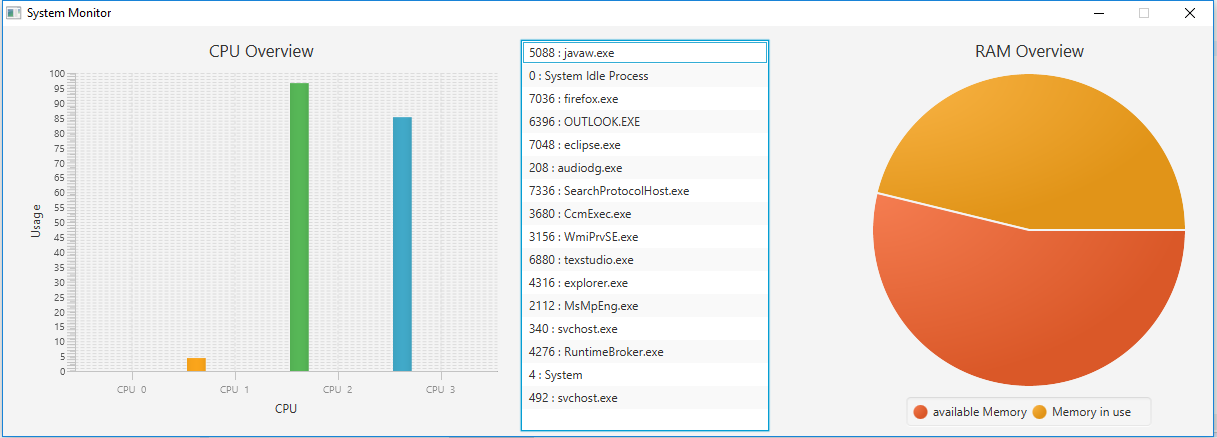
\includegraphics[width=1\textwidth]{Abb/sysmon}
	\caption{SystemMonitor Applikation}
	\label{pic:sysmon}
\end{figure}
In diesem Kapitel soll nun eine simple Anwendung beschrieben werden, die einige der zuvor geschilderten Methoden implementiert. Augenmerk liegt hier auf der Erstellung von Observables und die weitere Verwendung dieser. Als Beispiel soll ein Systemmonitor dienen. Hierfür werden die aktuelle Auslastung der Kerne, die ausgeführten Prozesse sortiert nach der CPU-Auslastung sowie der aktuell genutzte Arbeitsspeicher ausgelesen und auf einer Oberfläche dargestellt. Die Implementierung wurde mit Java 8u121 und RxJava 2.0.8 realisiert. Zusätzlich kamen noch die Bibliotheken JavaFX 8, RxJavaFX 2.0.2 sowie Oshi 3.4.0 zum Einsatz \cite{rxajavafx}, \cite{oshi}. Das Bild \ref{pic:sysmon} zeigt die fertige Applikation.
\section{Klassenbeschreibung SystemProvider}
Um sicherzustellen das die geforderten Daten des Systemmonitors verfügbar sind, wurde das ISystemProvider-Interface implementiert. 
\lstinputlisting[linerange={7-19}, float=hbt, caption={ISystemProvider-Interface}, label=lst:interface]{../SystemMonitor/src/main/java/provider/ISystemProvider.java} 
Listing \ref{lst:interface} zeigt die zu implementierenden Methoden des Interfaces. Die festen Größen, wie die Anzahl der Kerne und der verfügbare Arbeitsspeicher, werden als primitive Datentypen zur Verfügung gestellt. Die variablen Werte, also CPU-Auslastung, Prozesse und genutzter Speicher werden durch Observables repräsentiert. Die Implementierung dieser Methoden wurden in der Klasse SystemProvider vorgenommen.Verwendung findet hier das Oshi-Framework. Dieses bietet eine Schnittstelle um auf Systeminformationen außerhalb der JVM zuzugreifen. Als Einstiegspunkt dient immer ein Objekt der SystemInfo-Klasse. Dieses bietet die weiteren Informationen über das Betriebssystem oder die verwendete Hardware der Maschine. Der SystemProvider wurde als Singleton implementiert, wodurch auch nur eine Instanz der SystemInfo-Klasse verwendet wird, um die spezifischen Systeminformationen abzurufen. Interessant ist hier die Implementierung von den Methoden \textit{fetchCpuValues()}, \textit{getAvailableMemory()} und \textit{getProcesses()}. 
\subsection{List< Observable<Double> > fetchCpuValues()}
\lstinputlisting[linerange={45-56}, float=hbt, caption={SystemProvider - Implementierung der fetchCpuValues()-Methode}, label=lst:fetch]{../SystemMonitor/src/main/java/provider/SystemProvider.java} 
Die Implementierung der \textit{fetchCpuValues()}-Methode ist in Listing \ref{lst:fetch} zu sehen. Die sich ändernden Werte liegen als Double vor und repräsentieren die Stelle, welche beobachtet werden soll. Durch das Iterieren über die Anzahl der vorhandenen Kerne wird für jeden Kern ein separates Interval-Observable instanziiert. Die Taktung des Intervalls liegt bei einer Sekunde. Der vom Intervall generierte Wert wird vernachlässigt. Jedoch wird der Takt genutzt, um eine Abfrage über die aktuelle Auslastung eines Kerns durchzuführen. Bei einem 4-Kern Prozessor wird also eine Liste mit vier Observables von der Methode zurück geliefert. Da es sich um \textit{Cold Oservables} handelt, werden zu diesem Zeitpunkt noch keine Werte ausgeben. Noch zu erwähnen ist, dass ein Scheduler genutzt wird, um diesen Vorgang durchzuführen. Somit wird nicht der Thread der möglichen Subscriber verwendet, was ein Blockieren verhindern soll. 
\subsection{Observable<Long> getAvailableMemory()}
In Listing \ref{lst:memorymethod} sieht man die Implementierung der Methode um den aktuell verfügbaren Arbeitsspeicher auszulesen. Die Abfrage des Werts wird wieder mit einem Intervall durchgeführt und die Werte werden durch ein Observable repräsentiert. Auch hier wird wieder der Computation-Scheduler als Threadpool verwendet. Bis auf die Flexibilität der Kernanzahl ist das Vorgehen der Datenabfrage somit identisch zur \textit{fetchCpuValues}-Methode. Somit wird hier notwendigerweise nur ein einzelnes Observable zurück gegeben.
\lstinputlisting[linerange={64-68}, float=hbt, caption={SystemProvider - Implementierung der getAvailableMemory()-Methode}, label=lst:memorymethod]{../SystemMonitor/src/main/java/provider/SystemProvider.java} \newpage
\subsection{Observable< List<String> > getProcesses()}
\lstinputlisting[linerange={76-97}, float=hbt, caption={SystemProvider - Implementierung der getProcesses()-Methode}, label=lst:processmethod]{../SystemMonitor/src/main/java/provider/SystemProvider.java}
Die in Listing \ref{lst:processmethod} gezeigte Methode liefert ebenfalls ein Observable-Objekt zurück. Unterschied zu den beiden anderen Methoden ist hier jedoch, dass nicht nur ein Wert beobachtet wird, sondern die komplette Liste der Prozesse. Zusätzlich zum getakteten Aufruf der getProcesses()-Methode der SystemInfo-Klasse wird hier die Datenrepräsentation der Objekte geändert. Durch die Funktion \textit{func} wird aus den einzelnen Prozessen eine Liste bestehend aus der PID(ProcessID) sowie dem Prozessnamen erstellt, parametrisiert auf den Datentyp String zur einfacheren Weiterverarbeitung. Die im Observable enthaltene Liste beinhaltet 16 Prozesse sortiert nach der CPU-Auslastung. \newpage
\section{Klassenbeschreibung MainApplication}
Der bisherige Teil der Implementierung hat nur die Datenbeschaffung erledigt, es fehlt die Darstellung dieser Daten auf der Oberfläche. Hierzu dient die Klasse \textit{MainApplication}. Durch das JavaFX-Framework kann eine einfache Oberfläche implementiert werden. Durch das Erweitern der Klasse mit der abstrakten Klasse \textit{Application} des JavaFX-Frameworks, muss die \textit{start()}-Methode von der MainApplication-Klasse implementiert werden. Diese wird in der Main-Methode, welche ebenfalls in dieser Klasse untergebracht ist, aufgerufen, was zum Start der Anwendung führt. Innerhalb dieser Methode wird die Basis für die graphische Darstellung in Form der ersten \textit{Stage} gelegt. Auf dieser Stage werden alle Elemente, die dargestellt werden sollen, in einem Wurzelobjekt zusammengeführt. 
\lstinputlisting[linerange={37-51}, float=hbt, caption={MainApplication - Implementierung der start()-Methode}, label=lst:mainstart]{../SystemMonitor/src/main/java/application/MainApplication.java} 
Wie dies genau geschieht wird in Listing \ref{lst:mainstart} beschrieben. Mit der BorderPane als Basislayout wird ein Wurzelelement der Oberfläche geschaffen. Darauf werden horizontal angeordnet die eigentlichen Knoten(Nodes) festgelegt. Die Anordnung wird durch die verwendete \textit{HBox} übernommen. Die statischen Methoden \textit{createBarChart()}, \textit{createProcessList()} und \textit{createPieChart()} sind die Methoden, auf welche das eigentliche Augenmerk gerichtet wird, denn in diesen Methoden werden die Observables der vorangegangenen SystemProvider-Klasse verwendet. 
\subsection{Node createBarChart()}
\lstinputlisting[linerange={53-55, 68-79}, float=hbt, caption={MainApplication - Auszug aus der Implementierung der createBarChart()-Methode}, label=lst:barchartmethod]{../SystemMonitor/src/main/java/application/MainApplication.java} 
Diese Methode liefert einen Knoten von Typ BarChart(Balkendiagramm) zurück. Die BarChart arbeitet mit Serien von Daten die innerhalb des Diagramms dargestellt werden. Jede Serie besteht wiederum aus eine Menge von Daten mit jeweils einem \textit{x} und einem \textit{y} Wert. Die Serien werden von dem BarChart-Objekt in einer \textit{ObservableList} verwaltet. Dieser Datentyp stammt aus der JavaFX-Bibliothek und bietet die Möglichkeit die Liste von Daten zu beobachten und bei Änderung zu reagieren. Die Reihenfolge der Beobachtung der Datenänderungen ist gestaffelt. Für jedes Observable welches einen Kern und somit dessen aktuelle Auslastung repräsentiert, wird in einer separaten Serie gespeichert. Jede dieser Serien enthält einen Datensatz. In der Hilfsmethode \textit{setObservableChartData()} wird dieser Schritt durchgeführt wie es auch in Listing \ref{lst:helpermethod} dargestellt ist. 
\lstinputlisting[linerange={ 81-90}, float=hbt, caption={MainApplication - zusätzliche Hilfmethode setObservableChartData()}, label=lst:helpermethod]{../SystemMonitor/src/main/java/application/MainApplication.java} 
\\ \\ Der verantwortliche Datensatz der Serie subscribed dem Observable welches den aktuellen CPU-Wert propagiert. Somit enthält die Serie eine Datensatz mit sich ständig ändernden Daten. Diese Serie wird nun in der ObservableList abgelegt. Sind Serien für jeden der Kerne erstellt, wird die Liste als Datensatz dem Balkendiagramm übergeben. Findet nun eine Wertänderung statt, wird diese auf dem \textit{JavaFxScheduler.platform()}-Thread ausgeführt. Dieser Thread repräsentiert die Änderungen auf der Oberfläche. Somit wird bei jeder Wertänderung die Serie des Balkendiagramms aktualisiert. Die Implementierung der \textit{createBarChart()}-Methode und die Verwendung der Hilfsmethode zeigt Listing \ref{lst:barchartmethod}. In der \textit{for()}-Schleife wird für jeden Kern die Hilfsmethode ausgeführt und eine Serie mit Daten zurück geliefert. Diese wird der ObservableList hinzugefügt, welche wiederum als Datensatz des BarCharts verwendet wird.
\subsection{Node createPieChart()}
\lstinputlisting[linerange={92-94,101-105, 107-111, 114-115}, float=hbt, caption={MainApplication - Auszug aus der Implementierung der createPieChart()-Methode}, label=lst:piechartmethod]{../SystemMonitor/src/main/java/application/MainApplication.java} 
Die Auslastung des RAM wird als PieChart(Kreisdiagramm) dargestellt. Auch hier werden die Daten wieder in einer ObservableList parametrisiert auf den Datentyp Data abgelegt, welcher von der PieChart-Bibliothek zur Verfügung gestellt wird. In diesem Beispiel besteht der Kreis nur aus zwei Werten, dem genutzten und dem noch verfügbaren RAM. Das Observable erhält die Methode des SystemProviders über die Verwendung der SystemProvider-Instanz. Da die beiden Werte immer zusammen den Kreis komplett ausfüllen, also 100\% des RAM repräsentieren, werden die beiden Werte in einer Subscription aktualisiert. Auch hier erhält das PieChart die ObservableList mit den beiden Werten. Die Wertänderung wird wieder auf dem JavaFxScheduler-Threadpool ausgeführt, um die Wertänderungen an die GUI zu publizieren. Listing \ref{lst:piechartmethod} zeigt diese Implementierung. Als Node für die GUI wird die PieChart von der Methode zurückgegeben.
\subsection{Node createProcessList()}
\lstinputlisting[linerange={117-125}, float=hbt, caption={MainApplication - Implementierung der createProcesses()-Methode}, label=lst:getprocessesmethod]{../SystemMonitor/src/main/java/application/MainApplication.java}
Die Prozessliste wird von einem Node des Types ListView(Listenansicht) auf der Benutzeroberfläche repräsentiert. Die \textit{getProcesses()}-Methode des Systemproviders liefert wieder das Observable, was jede Sekunde die Liste der Prozesse über das Oshi-Framework abfragt. Die Beobachtung findet über die vollständige Liste statt, somit findet auch die Subscription an diesem Observable-Objekt statt. Die Daten der ListView werden ebenfalls in einer ObservableList verwaltet. Innerhalb der Subscription wird somit die Liste des Providers in eine ObservableList transformiert und als Einträge in die ListView hinzugefügt. 
Die konkrete Implementierung findet sich in Listing \ref{lst:getprocessesmethod}.
\section{Beschreibung des Beispiels}
Das Beispiel implementiert mehrere Methoden nach den Prinzipien des Reactive Programming. Die Systeminformationen werden über die vom Oshi-Framework zu Verfügung stehenden Methoden bezogen. Dies geschieht nach dem Pull-Verfahren, also für jede Abfrage der Daten muss ein separater Aufruf der Methode stattfinden. Hierfür dient die Instanziierung der Observables als Intervall. Diese Observables werden alle in einem Thread des RxJava eigenen \textit{Schedulers.computation()} Threadpool gestartet, sobald eine Subscription registriert wird. Somit handelt es sich hier um Cold Observables. Betrachtet man die Methode für das Erstellen der Observables für die Auslastung der einzelnen Kerne stellt man fest, dass die Intervalle unabhängig voneinander starten. Somit findet die Aktualisierung der Werte der unterschiedlichen Kerne asynchron und nebenläufig statt. Die Datenaktualisierung der GUI muss auf dem MainThread der JavaFX-Application ausgeführt werden. Um diesen Thread nur für die vorgesehenen Aktualisierungen zu verwenden, wird bei jeder der Methoden zum Erstellen der unterschiedlichen Nodes der \textit{JavaFxScheduler.platform()} Threadpool verwendet und zwar nur für die relevanten Datenänderungen und nicht für zusätzliche, von der GUI unabhängige, Aufgaben. Somit muss die Funktionalität der \textit{observOn()}-Methode für die jeweilige Subscription genutzt werden, sodass die Berechnung und Datenbeschaffung außerhalb und die Änderung der beobachteten Daten der Oberflächenelemente innerhalb des MainThreads der Application ausgeführt werden. Durch die Vielfalt der RxJava-Bibliothek kann dieses Beispiel nur einige Aspekte dieser Bibliothek abdecken, veranschaulicht aber zumindest den grundsätzlichen Umgang mit Observables innerhalb einer Applikation.
